%! TEX program = xelatex
\documentclass{article}
\usepackage[UTF8]{ctex}
\usepackage[margin=1in]{geometry}
\usepackage[hidelinks]{hyperref}
\usepackage{amsmath}
\usepackage{lmodern}
\usepackage{footnote}
\usepackage{graphicx}
\usepackage{float}
\usepackage{placeins}
\usepackage{xparse}
\usepackage{listings}
\usepackage{fontspec}

\graphicspath{{res/}}

\setmonofont[
    Contextuals={Alternate},
    ItalicFont = Fira Code      % to avoid font warning
]{Fira Code}

\DeclareDocumentCommand{\inputCodeSetLanguage}{ m }{
    \lstset{
        basicstyle=\small\ttfamily,
        language={#1},
        tabsize=4,
        showstringspaces=false,
        breaklines=true,
        frame=shadowbox,
        framexleftmargin=10mm,
        rulesepcolor=\color{black},
        numbers=left,
        xleftmargin=4em,
    }
}


\title{基于k-NN的人脸识别算法}
\author{计卓1501 胡思勖 U201514898}

\begin{document}
\maketitle

\paragraph{摘要}
\label{par:zhai_yao_}
\par 在信息化高速发展的今天,人们对于一个快速的身分验证方法的需求越来越广泛,从智能手机到门禁,人脸识别似乎成为了一个快速且行之有效的认真途径。本文尝试实现一个基于k-NN的人脸识别算法,并从中一窥现代人脸识别技术的完整面貌。

\section{综述}
\label{sec:zong_shu_}

\subsection{数据集}
\label{sub:shu_ju_ji_}
\par 本实验的数据集采用了剑桥大学Olivetti Research实验室1992年4月到1994年4月摄制的人脸照片。数据集包含40个不同的对象,每一个对象10张不同的人脸照片。所有的照片都是在黑暗的背景下拍摄的,同一个对象的照片有些许不同,包括一些光照的不同以及面表情和面部细节的不同。所有的文件都是pgm格式的,便于读取。同一个对象的照片存于同一个文件夹中,编号s1\textasciitilde s40,同一个对象的不同照片分别编号为1.pgm\textasciitilde 10.pgm。

\subsection{算法}
\label{sub:suan_fa_}
\par 在本实验中,主要采用了k-NN算法对于人脸进行归类识别,并辅以其他的算法来检测识别的性能。k-NN算法的过程如下:
\begin{enumerate}
    \item 遍历训练数据集,计算预测样本与其他每一个样本点的距离,按照由近到远排序;常用距离有曼哈顿距离、欧式距离和闵可夫斯基距离。
    \item 需要预先定义一个超参数参数k值,k是一个大于或等于1的整数,表示纳入投票决策的样本数。
    \item 统计离预测样本最近的k个样本,统计各个分类数目,返回数量最多的类的标签作为预测值。
\end{enumerate}
\par 使用数学语言描述如下:
\begin{itemize}
    \item 输入:训练数据集
        \[T={(x_1,y_1),(x_2,y_2),...,(x_N,y_N)}\]
        其中,\(x_i \in \mathcal{X} \subseteq R^n\)为实例的特征向量,\(y_i \in \mathcal{Y}=\{c_1,c_2,...,c_k\}\)为实例的类别,\(i=1,2,...,N\);实例特征向量\(x\);
    \item 输出: 实例x所属的类y
        \begin{enumerate}
            \item 根据给点的距离度量,在训练集\(T\)中找出与\(x\)最近邻的\(k\)个点,涵盖着\(k\)个点的领域,记为\(N_k(x)\);
            \item 在\(N_k(x)\)中根据分类决策规则(如多数表决),决定\(x\)的类别\(y\):
        \end{enumerate}
        \[y=\mathop{argmax}_{c_j} {\sum}_{x_i \in  N_k(x)} \; I(y_i=c_j) , i=1,2,...,N\]
\end{itemize}

\par 如图\ref{fig:knn}所示,如果k=3,则离绿球最近的三个样本中,三角形最多(2个),这时预测标签会返回三角形,如果k=5,那么正方形有3个,这时结果就变成了正方形。k值的选取,需要对通过目标的理解,尝试等方式确定。


\begin{figure}[htpb]
    \centering
    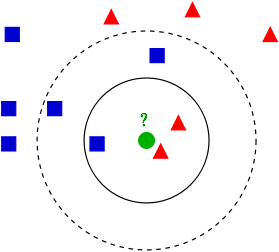
\includegraphics[width=0.4\linewidth]{knn.png}
    \caption{k-NN分类示例}
    \label{fig:knn}
\end{figure}
\FloatBarrier

\section{数据预处理}
\label{sec:shu_ju_yu_chu_li_}
\par 预处理是人脸识别过程中的一个重要环节。输入图像由于图像采集环境的不同,如光照明暗程度以及设备性能的优劣等,往往存在有噪声,对比度不够等缺点。另外,距离远近,焦距大小等又使得人脸在整幅图像中间的大小和位置不确定。为了保证人脸图像中人脸大小,位置以及人脸图像质量的一致性,必须对图像进行预处理。
\par 人脸图像的预处理主要包括人脸扶正,人脸图像的增强,以及归一化等工作。人脸扶正是为了得到人脸位置端正的人脸图像;图像增强是为了改善人脸图像的质量,不仅在视觉上更加清晰图像,而且使图像更利于计算机的处理与识别。归一化工作的目标是取得尺寸一致,灰度取值范围相同的标准化人脸图像。以下是本实验尝试过的预处理方法:
\begin{enumerate}
    \item 直方图均衡:直方图是一种点操作,它逐点改变图像的灰度值,尽量使各个灰度级别都具有相同的数量的像素点,使直方图趋于平衡。直方图均衡可以使输入图像转换为在每一个灰度级上都有相同像素点数的输出图像(即输出的直方图是平的)。这对于图像比较或分割是十分有用的。
    \item 中值滤波: 无论是直接获取的灰度图像,还是由彩色图像转换得到的灰度图像,里面都有噪声的存在,噪声对图像质量有很大的影响。进行中值滤波不仅可以去除孤点噪声,而且可以保持图像的边缘特性,不会使图像产生显著的模糊,比较适合于实验中的人脸图像。
\end{enumerate}
\par 然而由于本实验是基于k-NN算法的,其本质是计算图像每个对应点的距离和,因此使用这些提取特征和消去噪声的方法不一定对于算法的结果产生正面的影响。在实验中发现,不进行任何预处理的效果实际上是最好的。推测是由于原图片已经是在控制了较多变量环境下拍摄,已经保留了必要的信息而额外信息很少,经过这些预处理后反而有一定的信息损失而导致识别率降低。

\section{人脸识别算法实现}
\label{sec:tui_jian_suan_fa_shi_xian_}
\par 采用基于k-NN算法的人脸识别算法流程图如图\ref{fig:flow}所示。首先将训练数据加入训练数据集中,此处将每一个对象的输入数据分为训练数据和测试数据,而仅将训练数据预处理后加入数据集中。接下来直接执行k-NN算法,将测试数据与每一个训练数据集中的数据进行比对,并取前k个数据对应的标签中出现次数最多的作为测试数据的标签。

\begin{figure}[htpb]
    \centering
    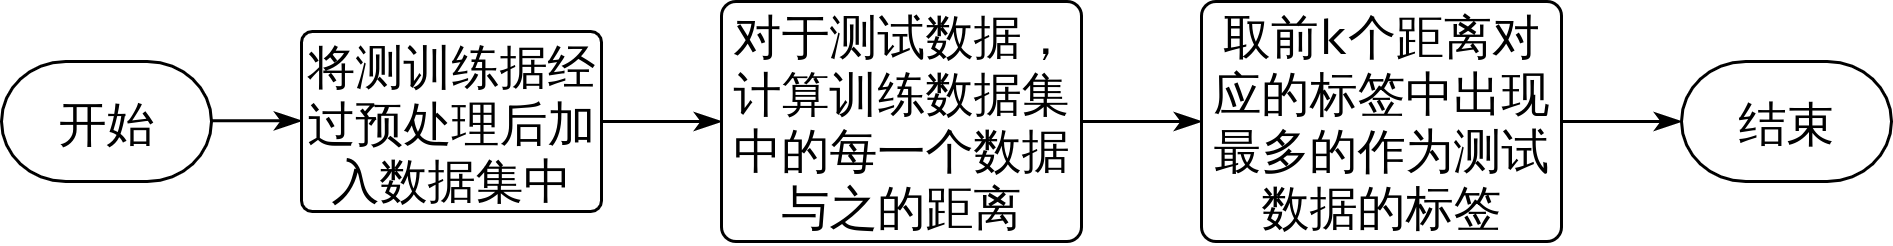
\includegraphics[width=0.8\linewidth]{flow.png}
    \caption{人脸识别算法基本流程}
    \label{fig:flow}
\end{figure}

\par 其中,在对于测试数据与训练数据的距离进行计算时,有多种计算方法,常用的计算方法有三种,分别为曼哈顿距离、欧氏距离和闵可夫斯基距离。其中,曼哈顿距离与欧氏距离均为闵可夫斯基距离的特例。
\par 设特征空间\(\mathcal{X}\)是\(n\)维实数向量空间\(R_n\), \(x_i,x_j\in X\), \(x_i,x_j \in \mathcal{X}, \quad x_i=(x_i^{(1)},x_i^{(2)},...,x_i^{(n)})^T\), \(x_i,x_j\)的\(L_p\)距离定义为:
\[L_p(x_i,x_j) = (\sum_{l=1}^{n} \; |x_i^{(l)}-x_j^{(l)}|^p)^{\frac{1}{p}}, p\ge 1\]

\par 当\(p=1\)时,称为曼哈顿距离:
\[L_1(x_i,x_j)= \sum_{l=1}^{n} |x_i^{(l)}-x_j^{(l)}|\]

\par 当\(p=2\)时,称为欧式距离:
\[L_2(x_i,x_j) = (\sum_{l=1}^{n} \; |x_i^{(l)}-x_j^{(l)}|^{2})^{\frac{1}{2}}\]

\par 当\(p=\infty\)时,它是各个坐标距离的最大值:
\[L_{\infty}(x_i,x_j)= \mathop{max}_l \; |x_i^{(l)}-x_j^{(l)}|\]

\par 此外,还有余弦距离、Jaccard相似系数等多种距离的计算方法。而为了便于实现,同时考虑到效果,性能方面的原因,在本实现中采用了欧拉距离作为最终的距离计算方法。
\par 为了便于取前k个距离,维护一个小根堆,在每次进行距离计算时将距离以及标签插入小根堆中,并在最后从小根堆的堆顶弹出k个数据。

\section{算法测试}
\label{sec:suan_fa_ce_shi_}
\par 对于单个图像进行测试,此处取k-NN参数\(k=10\),并将测试数据也加入训练集中,以验证程序功能上的正确性:此时测试图片与自身计算距离应为0,并且自身应为与自身距离最近的图片。其他的9张图片应该按照距离以降序排序。将所有的距离与匹配的标签个数输出后如图\ref{fig:output}所示。从图中可以初步判断程序的功能正常。此处,以s3/1.pgm为例进行测试,与其距离最近的图片是自身,随后是6个标签为s3的照片,然后是2个标签为s25的照片和1个标签为s38的照片。

\begin{figure}[htpb]
    \centering
    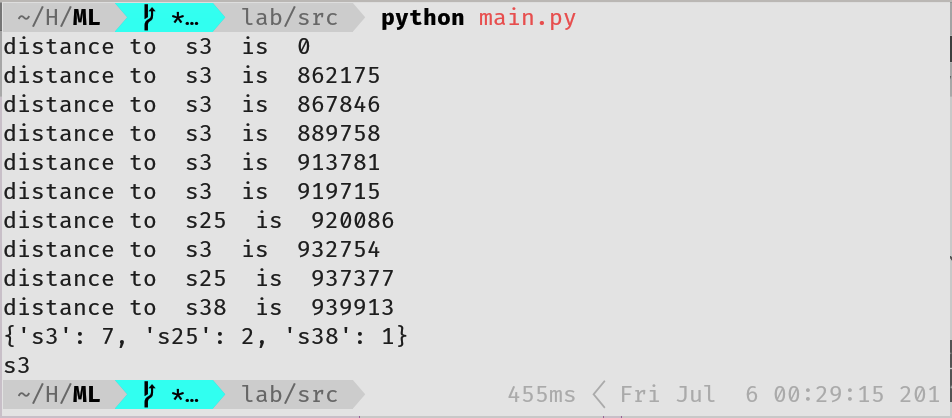
\includegraphics[width=0.95\linewidth]{output.png}
    \caption{对于s3/1.png进行测试的输出}
    \label{fig:output}
\end{figure}

\section{结果分析与评估}
\label{sec:jie_guo_fen_xi_yu_ping_gu_}

\subsection{评估方法}
\label{sub:ping_gu_fang_fa_}
\par 由于原始数据每一个人脸均有10张不同角度的照片,为了能够更好的利用数据,从有限的学习数据中获取尽可能多的有效信息,决定采用k折交叉验证的方式:在给定的样本空间中,拿出大部分样本作为训练集来训练模型,剩余的小部分样本使用刚建立的模型进行预测,并求这小部分样本的预测误差或者预测精度,同时记录它们的平均值。
\par 交叉验证从多个方向开始学习样本的,可以有效的避免陷入局部最小值,同时,可以在一定程度上避免过拟合问题。
\par 在本实验中,最终采用的k验证方法如图\ref{fig:flow2}所示。在每一次循环中采用具有循环编号的图片作为测试数据,其余为训练数据,使用图\ref{fig:flow}中的流程进行识别后将识别结果(是否正确)加入统计结果中。最后,输出统计结果。

\begin{figure}[htpb]
    \centering
    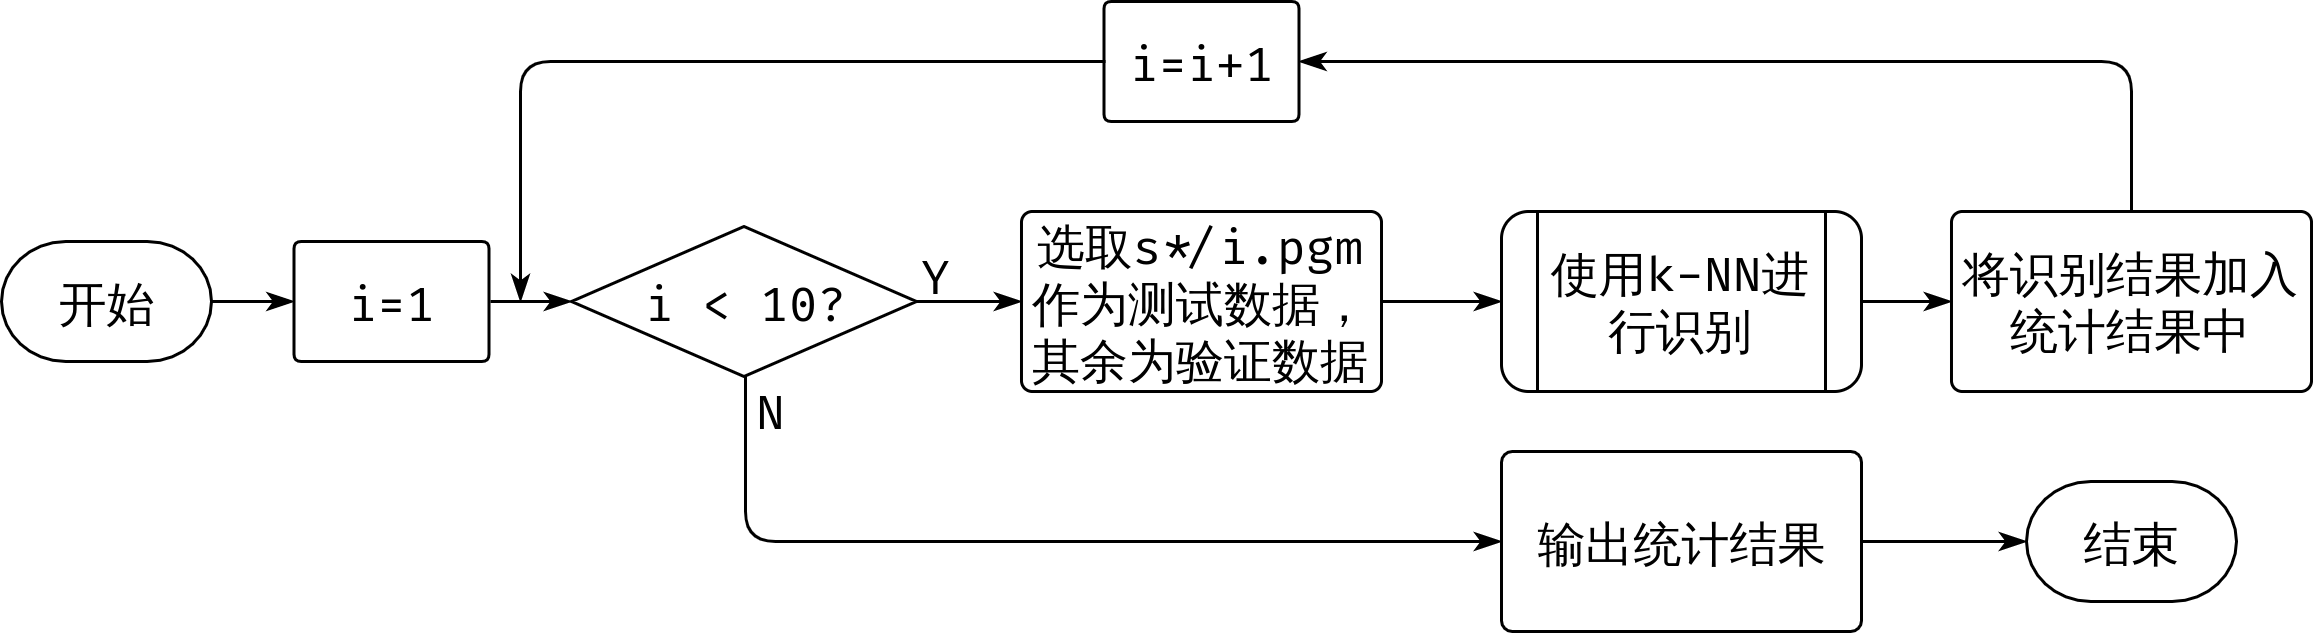
\includegraphics[width=0.95\linewidth]{flow2.png}
    \caption{测试程序流程}
    \label{fig:flow2}
\end{figure}
\FloatBarrier

\subsection{评估结果}
\label{sub:ping_gu_jie_guo_}

\par 取k=3,一测试的输出如图\ref{fig:output2}所示,从图中可以看出,识别的准确率为98.25\%。
\begin{figure}[htpb]
    \centering
    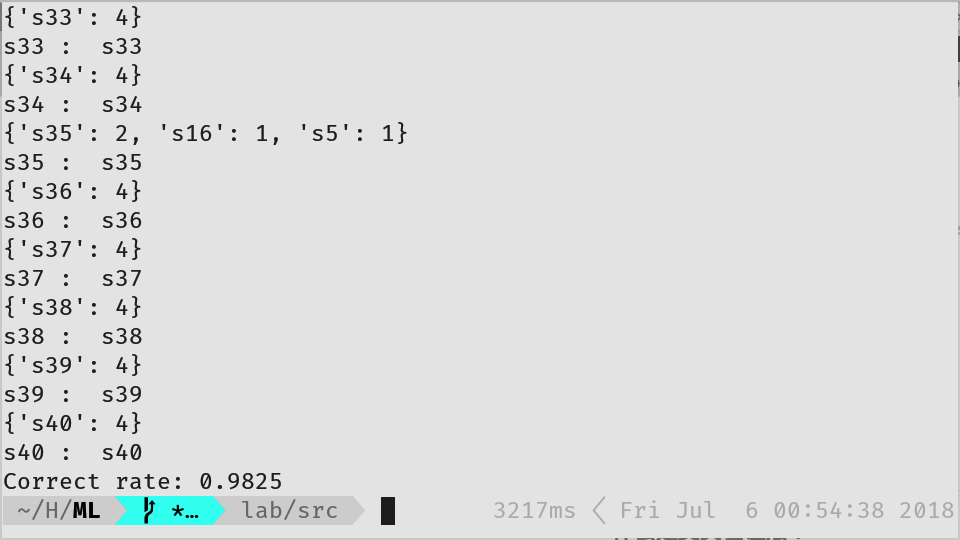
\includegraphics[width=0.95\linewidth]{output2.png}
    \caption{\(k=3\)时测试输出(部分)}
    \label{fig:output2}
\end{figure}

\par 就算法的结果来看,算法的性能还是较为不错的,对于k为其他值时,准确率如图\ref{fig:chart}所示。图为对于\(k=1\)\textasciitilde \(k=20\)的测试结果从图中可以看出,程序的正确率随着k的值上升而下降。这一结果是不具有普遍性的,但是对于本程序而言,选取一个较小的值对于测试结果有着正面的影响,在交叉验证下最高正确率可达99.5\%。

\begin{figure}[htpb]
    \centering
    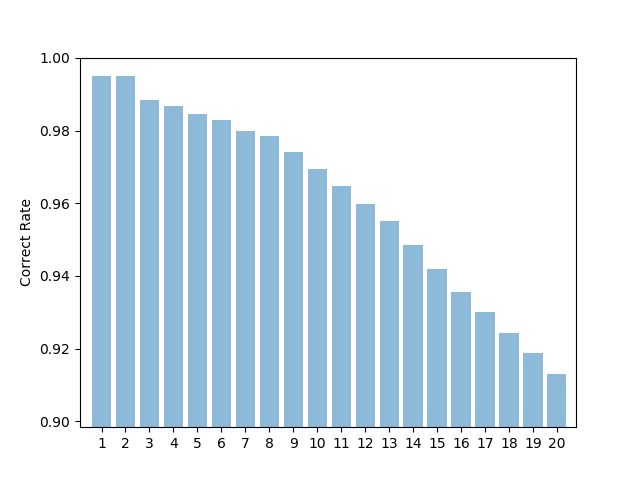
\includegraphics[width=0.8\linewidth]{chart.png}
    \caption{正确率与k的关系}
    \label{fig:chart}
\end{figure}

\FloatBarrier
\section{结语}
\label{sec:jie_yu_}
\par 此次实验基于k-NN算法实现了一个人脸识别,并达到了较高的准确率。k-NN是机器学习领域中一个十分基础的算法,然而此次实验表明它依然是一种行之有效的算法。对于40个对象的人脸识别准确率甚至达到了99.5\%。然而值得注意的是,这是基于输入数据是一个经过良好处理的数据集这一前提的。在实际的应用过程中,输出数据没用如此强的一致性,因此需要结合PCA、神经网络等算法来达到更好的效果。
\par 此外,这一实验也说明了预处理方法的重要性,对于本实验而言,最好的预处理方法是不进行任何预处理,而在其他的情况下,预处理是十分重要且必不可少的。对于图片的预处理能够极大地影响人脸识别的结果。

\section{源代码}
\label{sec:yuan_dai_ma_}
\inputCodeSetLanguage{python}
\lstinputlisting{../src/main.py}

\end{document}
